\newpage
{\color{gray}\hrule}
\begin{center}
\section{Rivelazione dei muoni cosmici }
\bigskip
\end{center}
{\color{gray}\hrule}
Dei raggi cosmici che raggiungono la superficie terrestre, i muoni $\mu^{\pm}$ rappresentano la quasi totalità, poichè hanno vita
media relativamente lunga ed essendo molto pesanti ($\approx $ 200 $m_e$) vengono poco frenati dalle interazioni in atmosfera.\\ Lo stesso kit SiPM descritto nel capitolo 2 può essere utilizzato anche per la rivelazione dei muoni cosmici, ma a differenza delle particelle $\beta^-$, per le quali è possibile effettuare spettroscopia completa, nel caso dei muoni si può parlare unicamente di frazione di energia depositata nel rivelatore, poiché essi non vengono completamente arrestati all’interno del materiale.
Lo scintillatore risulta quindi adatto anche alla rivelazione di particelle altamente energetiche (dell’ordine dei GeV), per le quali non si intende misurare l’energia totale, ma semplicemente rilevarne il passaggio.

Per ottenere uno spettro dell’energia depositata dai muoni, il rivelatore 
SiPM+scintillatore viene posizionato tra due scintillatori plastici, ciascuno 
accoppiato a un fotomoltiplicatore tramite fibra ottica.
La luce di scintillazione prodotta dal passaggio delle particelle ionizzanti 
viene così raccolta dai rispettivi fotomoltiplicatori e, nel caso di coincidenza temporale 
tra i due segnali, utilizzata come trigger esterno per il Digitizer.

\textit{Osservazione.} In questo caso non si utilizza come trigger esterno l’uscita DOUT della PSAU perché questa genera un segnale ogni volta che un impulso supera la soglia, includendo quindi anche segnali non associati al passaggio di un muone. Inoltre, a differenza del caso di una sorgente LED affrontata nel primo capitolo, il flusso
di muoni cosmici è molto basso e il loro rate è confrontabile con il \textit{dark count rate} del SiPM. Per questo motivo si sfrutta il segnale di coincidenza della \textit{Cosmic Box}, in quanto la probabilità che il rumore interno produca segnali coincidenti in entrambi i rivelatori è estremamente bassa.

\subsection{Spettro di energia depositata dai $\mu^\pm$}
Di seguito si riporta lo spettro dell'energia depositata dalle particelle acquisito in laboratorio.\\

\begin{figure} [H]
    \centering
    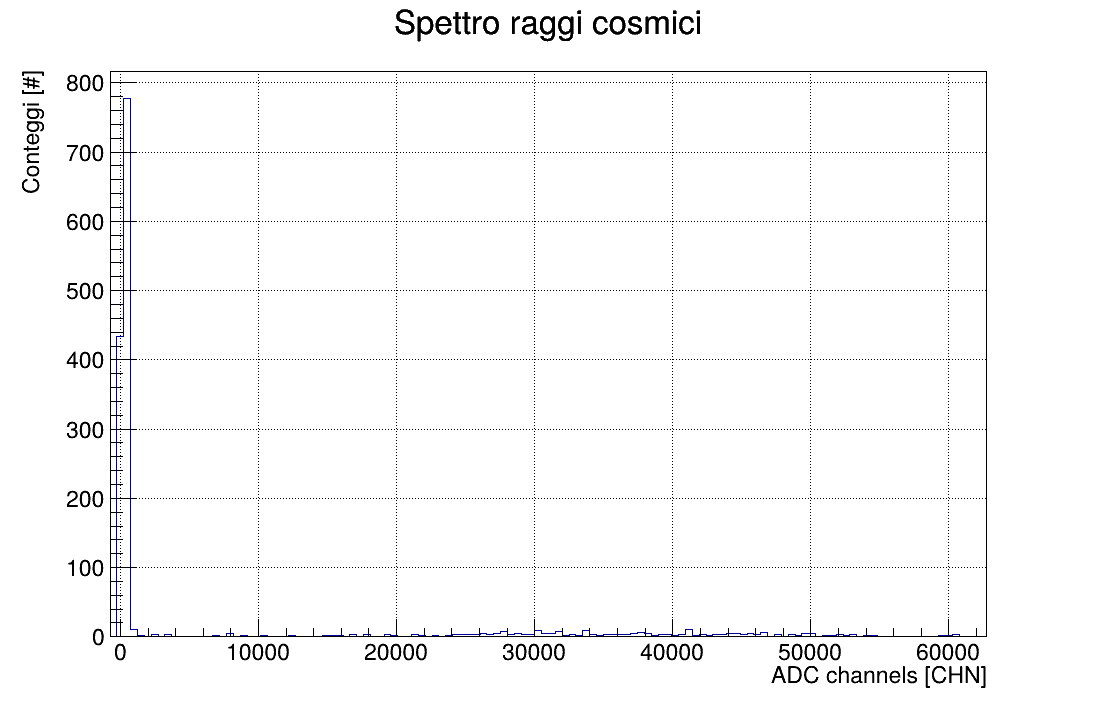
\includegraphics[width=0.62\linewidth]{fig2/raggi.png}
    \caption{ \footnotesize Istogramma di conteggi per numero di canale per i muoni cosmici completo ($G_{ampl}=28$dB e $V_{bias}=54V$).}
    \label{fig:raggi}
\end{figure}

Nel grafico \ref{fig:raggi} si osserva che, a causa della differenza di superficie attiva tra il SiPM e gli scintillatori esterni, il numero massimo di conteggi si registra in corrispondenza 
dello zero, ovvero quando la particella non attraversa anche il SiPM.

È inoltre presente un picco secondario di minore intensità (vedi figura \ref{fig:raggizoom}), intorno a 30000 CHN, associato agli eventi in cui la particella attraversa effettivamente il rivelatore centrale, depositando energia nello scintillatore. Come evidenziato dal grafico, la distribuzione dei conteggi presenta un andamento gaussiano nella regione a sinistra del picco, mentre risulta allungata alla sua destra. \\ Tale asimmetria è dovuta al fatto che le particelle incidenti con angoli diversi dalla perpendicolare percorrono una distanza maggiore all’interno dello scintillatore, depositando quindi più energia. L’andamento gaussiano nella regione sinistra può invece essere interpretato come il risultato delle fluttuazioni statistiche intrinseche.

\begin{figure} [H]
    \centering
    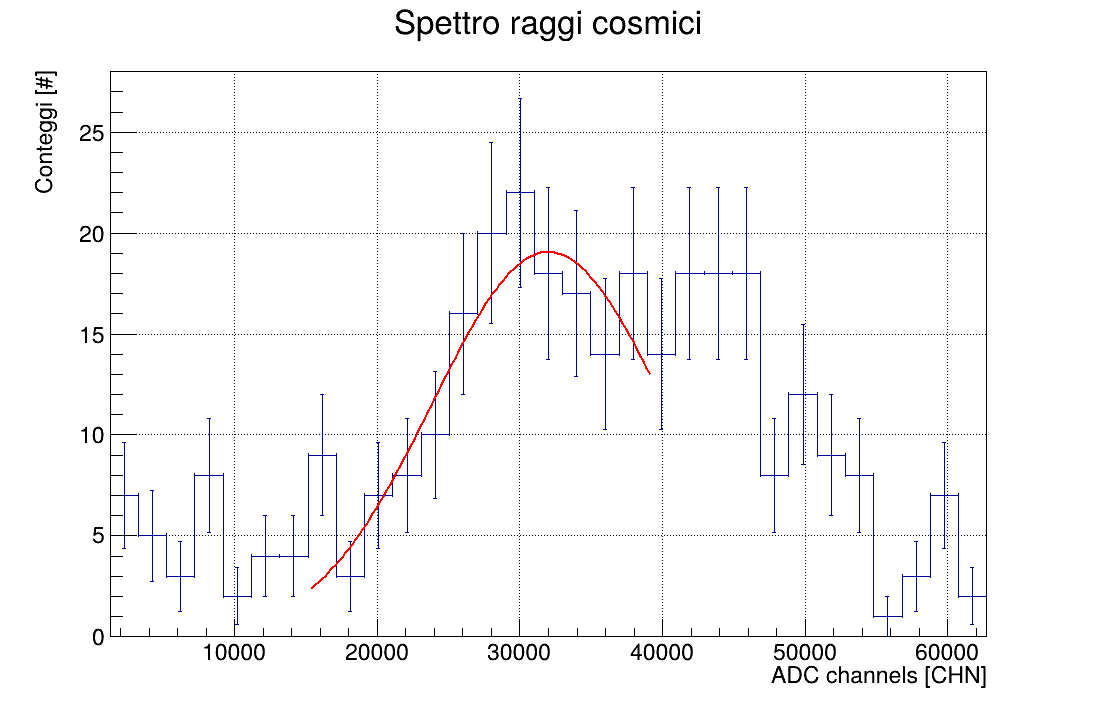
\includegraphics[width=0.65\linewidth]{fig2/raggi_zoom.png}
    \caption{ \footnotesize \footnotesize Istogramma di conteggi per numero di canale per i muoni cosmici con zoom sulla distribuzione di energia ($G_{ampl}=28$dB e $V_{bias}=54V$) e fit gaussiano: paramentri estratti $ \langle CHN\rangle = (32.0  \pm  1.6 )\cdot10^3\text{ CHN}$  e $ \sigma_{CHN} = ( 8.1 \pm 1.5 )\cdot10^3 \text{CHN}$, $\chi^2 =8$ e d.o.f.=9.}
    \label{fig:raggizoom}
\end{figure}
Dal fit gaussiano a sinistra del picco si estraggono valore medio e rispettiva deviazione standard, nonché la sua risoluzione: $$\langle \text{CHN} \rangle = ( 32  \pm  8  )\cdot10^3 \text{ CHN} $$ $$R_{CHN}= \frac{\sigma_\text{CHN}}{\langle\text{CHN}\rangle}= 0.25 \pm 0.05$$
Tramite il fattore di conversione $k_{Sr,eq}$, calcolato nella sezione 2.1.3, è possibile convertire $\langle \text{CHN} \rangle$ in energia depositata.
$$E_{DEP}=k_{Sr,eq}\cdot \langle CHN \rangle=( 1.6  \pm  0.5  ) \text{MeV}$$

\textit{Osservazione.} Come già accennato nella sezione 2.1.3, si utilizza $k_{eq}$ al posto di $k$ perché, nel caso dei raggi cosmici, le 
particelle non incidono sempre perpendicolarmente al rivelatore né attraversano per forza
il centro dello scintillatore. Al contrario, queste possono colpire la lastra in 
punti diversi e con angoli differenti, determinando una risposta del rivelatore 
che dipende dalla posizione di attraversamento.
Per tenere conto di questa non uniformità, si introduce quindi $k_{eq}$, che rappresenta il valore medio di $k$ nel caso in cui gli eventi siano distribuiti uniformemente su tutta la superficie dello scintillatore. \\

Infine, si verifica la legge di Bethe-Bloch per la perdita di energia, la quale prevede $$E_{DEP,att} = \frac{dE}{dx}x$$
dove $x$ è lo spessore dello scintillatore. 

Sapendo che $x=1\text{cm}$ e che per il polistirene si ha $\frac{dE}{dx}=2.06$ $\frac{MeV}{cm}$, si ottiene un valore atteso
$$E_{DEP,att} = 2.06 MeV $$ il quale risulta statisticamente compatibile con la stima sperimentale $E_{DEP}$.
